\documentclass[oneside, 11pt]{article}

\usepackage[T1]{fontenc}
\usepackage[utf8]{inputenc}
\usepackage[english]{babel}
\usepackage{enumerate}
\usepackage{isotope}


\usepackage{fouriernc}
\usepackage[detect-all, binary-units, separate-uncertainty=true,
            per-mode=symbol, retain-explicit-plus, retain-unity-mantissa=false]{siunitx}

\usepackage{setspace}
\setstretch{1.2}

\setlength{\parskip}{\smallskipamount}
\setlength{\parindent}{0pt}

\usepackage[headheight=14pt]{geometry}
\geometry{marginparwidth=0.5cm, verbose, a4paper, tmargin=3cm, bmargin=3cm,
          lmargin=2cm, rmargin=2cm}

\usepackage{float}

\usepackage[fleqn]{amsmath}
\numberwithin{equation}{section}
\numberwithin{figure}{section}

\usepackage{graphicx}
\graphicspath{{images/}{../../../images/}}

\usepackage{tikz}
\usetikzlibrary{shapes}
\usetikzlibrary{plotmarks}

\newcounter{Exercise}
\setcounter{Exercise}{1}
\usepackage{xcolor}
\definecolor{shadecolor}{gray}{0.9}
\usepackage{framed}
\usepackage{caption}

\usepackage{url}


\usepackage{fancyhdr}
\pagestyle{fancy}
\fancyhf{}
\rhead{\thepage}
\renewcommand{\footrulewidth}{0pt}
\renewcommand{\headrulewidth}{0pt}

\fancypagestyle{firststyle}
{
    \fancyhf{}
    \rhead{\thepage}
    \cfoot{\includegraphics[height=30pt]{HiSPARClogo}}
    \rfoot{\includegraphics[height=25pt]{CCbysa}}
    \lfoot{
\includegraphics[height=30pt]{NIKHEFlogo}}
    \renewcommand{\footskip}{50pt}
    \renewcommand{\footrulewidth}{0.1pt}
    \renewcommand{\headrulewidth}{0pt}
}

\newcommand{\figref}[1]{Figuur~\ref{#1}}

\newcommand{\hisparc}{\textsmaller{HiSPARC}\xspace}
\newcommand{\kascade}{\textsmaller{KASCADE}\xspace}
\newcommand{\sapphire}{\textsmaller{SAPPHiRE}\xspace}
\newcommand{\jsparc}{\textsmaller{jSparc}\xspace}
\newcommand{\hdf}{\textsmaller{HDF5}\xspace}
\newcommand{\aires}{\textsmaller{AIRES}\xspace}
\newcommand{\csv}{\textsmaller{CSV}\xspace}
\newcommand{\python}{\textsmaller{PYTHON}\xspace}
\newcommand{\corsika}{\textsmaller{CORSIKA}\xspace}
\newcommand{\labview}{\textsmaller{LabVIEW}\xspace}
\newcommand{\daq}{\textsmaller{DAQ}\xspace}
\newcommand{\adc}{\textsmaller{ADC}\xspace}
\newcommand{\hi}{\textsc{h i}\xspace}
\newcommand{\hii}{\textsc{h ii}\xspace}
\newcommand{\mip}{\textsmaller{MIP}\xspace}
\newcommand{\hisparcii}{\textsmaller{HiSPARC II}\xspace}
\newcommand{\hisparciii}{\textsmaller{HiSPARC III}\xspace}

\DeclareSIUnit{\electronvolt}{\ensuremath{\mathrm{e\!\!\:V}}}

\DeclareSIUnit{\unitsigma}{\ensuremath{\sigma}}
\DeclareSIUnit{\mip}{\textsmaller{MIP}}
\DeclareSIUnit{\adc}{\textsmaller{ADC}}

\DeclareSIUnit{\gauss}{G}
\DeclareSIUnit{\parsec}{pc}
\DeclareSIUnit{\year}{yr}



%document details
\author{N.G. Schultheiss \\ translated and adapted by K. Schadenberg}
\date{}
\title{Telescopes}


\begin{document}
\maketitle

\section{Introduction}
This module `Telescopes follows the module `Lenses' or `Grinding Lenses'. When you completed this module you should be able to make your own telescope and explain how it works.

\section{Types of telescopes}
Telescopes can be divided into two groups: refractors and reflectors. With a refractor telescope the light entering the telescope will first encounter a lens. In a reflector this is a mirror. The first optical element is called the objective. The objective is the closest to the object one is looking at.\footnote{Closest in the entire path of light, the objective in a reflector telescope might be at the back of the telescope!} The optical element closest to the eye is the eyepiece or ocular.

\subsection{Refractors}
The telescope used by Galileo Galilei during the renaissance was a refractor. The telescope used a convex objective and a concave ocular. This design is called a `Hollandse kijker' (Dutch viewer) or Galilean telescope, see figure \ref{fig:tel_gal}.

\begin{figure}\begin{center}
\begin{picture}(0,0)%
\includegraphics[scale=0.9]{Galilean}%
\end{picture}%
\setlength{\unitlength}{4144sp}%
%
\begingroup\makeatletter\ifx\SetFigFont\undefined%
\gdef\SetFigFont#1#2#3#4#5{%
  \reset@font\fontsize{#1}{#2pt}%
  \fontfamily{#3}\fontseries{#4}\fontshape{#5}%
  \selectfont}%
\fi\endgroup%
\begin{picture}(7764,1353)(79,-1423)
\end{picture}%
\caption{A Galilean telescope.}\label{fig:tel_gal}
\end{center}\end{figure}

\begin{shaded}
\textbf{Exercise \theExercise \stepcounter{Exercise}} : What way round is the image made by a Galilean telescope? Upside down or the right way up? Use the ray diagram of figure~\ref{fig:tel_gal} in your explanation.\end{shaded}

The Galilean telescope has a very limited field of view and, depending on the quality of the lenses, a number of pronounced optical abberation (faults or distortions in the image). Johannes Kepler suggested an improvement to the original design. He suggested using two convex lenses. Distortions of the image were still very common, but the field of view was much larger. Christaan Huygens improved the magnification and amount of (chromatic) aberations of this design by using two lenses to form the ocular (see figure~\ref{fig:tel_huy}).

\begin{figure}\begin{center}
\begin{picture}(0,0)%
\includegraphics[scale=0.75]{huygens}%
\end{picture}%
\setlength{\unitlength}{4144sp}%
%
\begingroup\makeatletter\ifx\SetFigFont\undefined%
\gdef\SetFigFont#1#2#3#4#5{%
  \reset@font\fontsize{#1}{#2pt}%
  \fontfamily{#3}\fontseries{#4}\fontshape{#5}%
  \selectfont}%
\fi\endgroup%
\begin{picture}(9384,1353)(79,-1423)
\end{picture}%
\caption{A Keplerian telescope with a Huygens ocular.}\label{fig:tel_huy}
\end{center}\end{figure}

\begin{shaded}
\textbf{Exercise \theExercise \stepcounter{Exercise}} : What way round is the image made by a Keplerian telescope? Upside down or the right way up? Use the ray diagram of figure~\ref{fig:tel_huy} in your explanation.\end{shaded}
\begin{shaded}
\textbf{Exercise \theExercise \stepcounter{Exercise}} :  Jesse Ramsden was able to further improve Huygens' design by changing the orientation of the lenses and their distances. Search for the Ramsden design and explain the differences.\end{shaded}

\subsection{Reflectors}
Isaac Newton, a contemporary of Huygens, used a mirror instead of a lens as objective in his telescope design. His was the first functional reflector telescope design (see figure~\ref{fig:tel_new}). The focal point of the mirror and eye piece are at the same place, this can be at the second (plane) mirror but is not necessary.

\begin{figure}\begin{center}
\begin{picture}(0,0)%
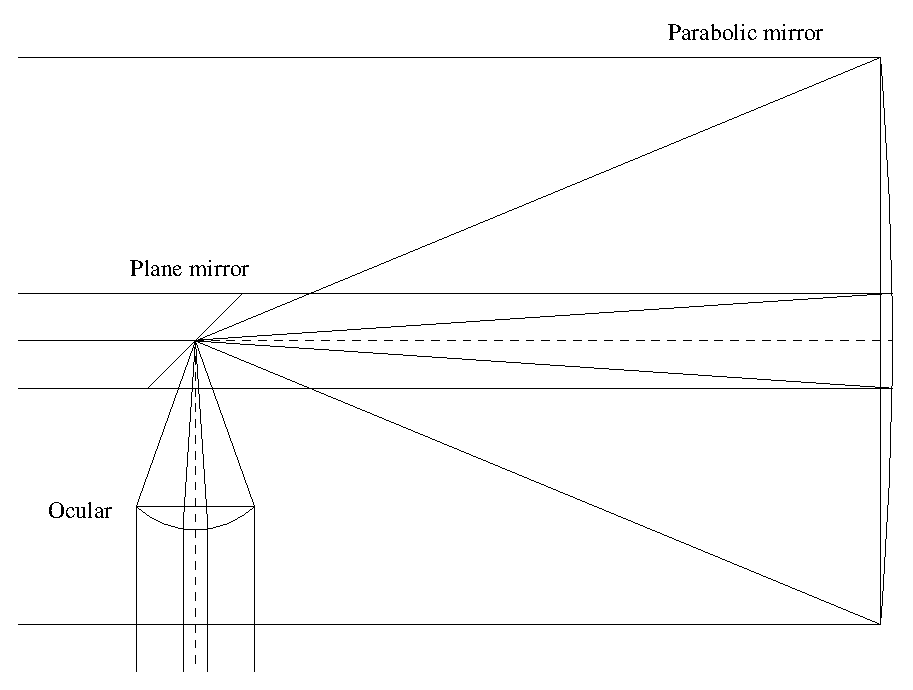
\includegraphics{newton}%
\end{picture}%
\setlength{\unitlength}{4144sp}%
%
\begingroup\makeatletter\ifx\SetFigFont\undefined%
\gdef\SetFigFont#1#2#3#4#5{%
  \reset@font\fontsize{#1}{#2pt}%
  \fontfamily{#3}\fontseries{#4}\fontshape{#5}%
  \selectfont}%
\fi\endgroup%
\begin{picture}(6684,4700)(79,-6193)
\end{picture}%
\caption{A Newton reflector type telescope.}\label{fig:tel_new}
\end{center}\end{figure}

\begin{shaded}
\textbf{Exercise \theExercise \stepcounter{Exercise}} : A large telescope is always a reflector, never a refractor, why?\end{shaded}

The astronomer Friedrich Wilhelm Herschel was building ever larger telescopes during the 17th and 18th century while studying the solar system and stars. With his investigation he came to the conclusion that our solar system was part of a larger galaxy, the Milky Way. Together with his sister Carline Lucretia Herschel he studied the orbits of asteroid. His son John Frederick William Herschel continued this work and started experimenting with photographic paper. A real astronomers family.

\section{Calculations}
\subsection{Magnification}
A number of the properties of a telescope can be calculated if we know the strength of the lenses or curvature of the mirrors. One of the most important properties is the magnification. In all the examples of telescopes in the previous section, the beam of light entering the telescope was drawn parallel, as was the beam exiting the telescope. Calculating the magnification of a telescope is therefore different than calculating the magnification of a single lens.

\begin{figure}\begin{center}
\setlength{\unitlength}{1mm}
\begin{picture}(150,50)
\put(0,15){\line(1,0){150}}
\put(55,0){\line(0,1){30}}
\put(54,32){Objective}
\put(56,26){A}
\put(56,10){$\mbox{O}_{\mbox{objective}}$}
\put(5,13){\line(0,1){4}}
\put(3,9){$\mbox{F}_{\mbox{objective}}$}
\put(125,0){\line(0,1){30}}
\put(124,32){Ocular}
\put(126,26){B}
\put(126,10){$\mbox{O}_{\mbox{ocular}}$}
\put(105,13){\line(0,1){4}}
\put(85,9){$\mbox{F}_{\mbox{objective}} = \mbox{F}_{\mbox{ocular}}$}
\put(145,13){\line(0,1){4}}
\put(143,9){$\mbox{F}_{\mbox{ocular}}$}
\put(0,14){\line(5,1){55}}
\put(55,25){\line(1,0){70}}
\put(125,25){\line(2,-1){25}}
\end{picture}
\caption{Schematic representation of a telescope.}\label{fig:tel_ray}
\end{center}\end{figure}

In figure \ref{fig:tel_ray} the path of light inside a telescope is represented schematically. If the light passes through the focal point before the objective, then inside the telescope it will travel parallel to the main axis of the telescope. When exiting at the ocular it will cross the focal point of the ocular. At the objective the light has a certain angle with the main axis: $ \angle \mbox{AF} _{\mbox{objective}} \mbox{O} _{\mbox{objective}} $. After the ocular there is a different angle: $ \angle \mbox{BF} _{\mbox{ocular}} \mbox{O} _{\mbox{ocular}} $.

\begin{align} \tan (\angle \mbox{BF}_{\mbox{ocular}} \mbox{O}_{\mbox{ocular}} ) &= \frac{\mbox{BO}_{\mbox{ocular}}}{\mbox{F}_{\mbox{ocular}}\mbox{O}_{\mbox{ocular}}} \\
\tan (\angle \mbox{AF}_{\mbox{objective}} \mbox{O}_{\mbox{objective}} ) &= \frac{\mbox{AO}_{\mbox{objective}}}{\mbox{F}_{\mbox{objective}}\mbox{O}_{\mbox{objective}}}
\end{align}
We divide the first equation by the second:
\begin{equation}
\frac{\tan (\angle \mbox{BF}_{\mbox{ocular}} \mbox{O}_{\mbox{ocular}} )}{\tan (\angle \mbox{AF}_{\mbox{objective}} \mbox{O}_{\mbox{objective}} )} = \frac{\left( \frac{\mbox{BO}_{\mbox{ocular}}}{\mbox{F}_{\mbox{ocular}}\mbox{O}_{\mbox{ocular}}} \right)}{\left( \frac{\mbox{AO}_{\mbox{objective}}}{\mbox{F}_{\mbox{objective}}\mbox{O}_{\mbox{objective}}} \right)}
\end{equation}
Using the fact that the two line segments AO$_{\mbox{objective}}$ and BO$_{\mbox{ocular}}$ have the same length:
\begin{equation}
\frac{\tan (\angle \mbox{BF}_{\mbox{ocular}} \mbox{O}_{\mbox{ocular}} )}{\tan (\angle \mbox{AF}_{\mbox{objective}} \mbox{O}_{\mbox{objective}} )} = \frac{\mbox{F}_{\mbox{objective}}\mbox{O}_{\mbox{objective}}}{\mbox{F}_{\mbox{ocular}}\mbox{O}_{\mbox{ocular}}}
\end{equation}

For small angles the tangent of an angle is almost the same as the angle in radians. We apply this simplification (linearisation) to the previous equation. We also know that the distance from F to O is the same as the focal distance $f$:
\begin{equation}
\frac{\angle \mbox{BF}_{\mbox{ocular}} \mbox{O}_{\mbox{ocular}} }{\angle \mbox{AF}_{\mbox{objective}} \mbox{O}_{\mbox{objective}} } = \frac{f_{\mbox{objective}}}{f_{\mbox{ocular}}}
\end{equation}
\begin{equation} \mbox{Angular magnification} = \frac{f_{\mbox{objective}}}{f_{\mbox{ocular}}} \end{equation}

\begin{shaded}
\textbf{Exercise \theExercise \stepcounter{Exercise}} : Christiaan Huygens built multiple telescopes. The telescope he used when he discovered the moon Titan had a objective with a focal length $f_{\mbox{objective}}=12~\mbox{feet}$ and a eye piece with a focal length $f_{\mbox{ocular}}=3~\mbox{inch}$. Calculate the angular magnification of this telescope.\end{shaded}

\subsection{Resolution}
The angular magnification of a telescope is just one of its characteristics, however it is one that is rarely reported. This is because the eye piece of a telescope is easily replaced by a different one, changing the magnification in the process.

The diameter of the objective is far more important to astronomers. The diameter can be directly linked to the resolution, or accuracy, with which telescopes can observe celestial objects. When two stars are very close to each other, or when a planet orbits a star, the rays of light coming from both objects are almost parallel. The rule of thumb is that two beams of light can be separated (or distinguished) when the lightfronts differ more than one wave length at the top and bottom of the mirror.

\begin{figure}\begin{center}
\setlength{\unitlength}{1mm}
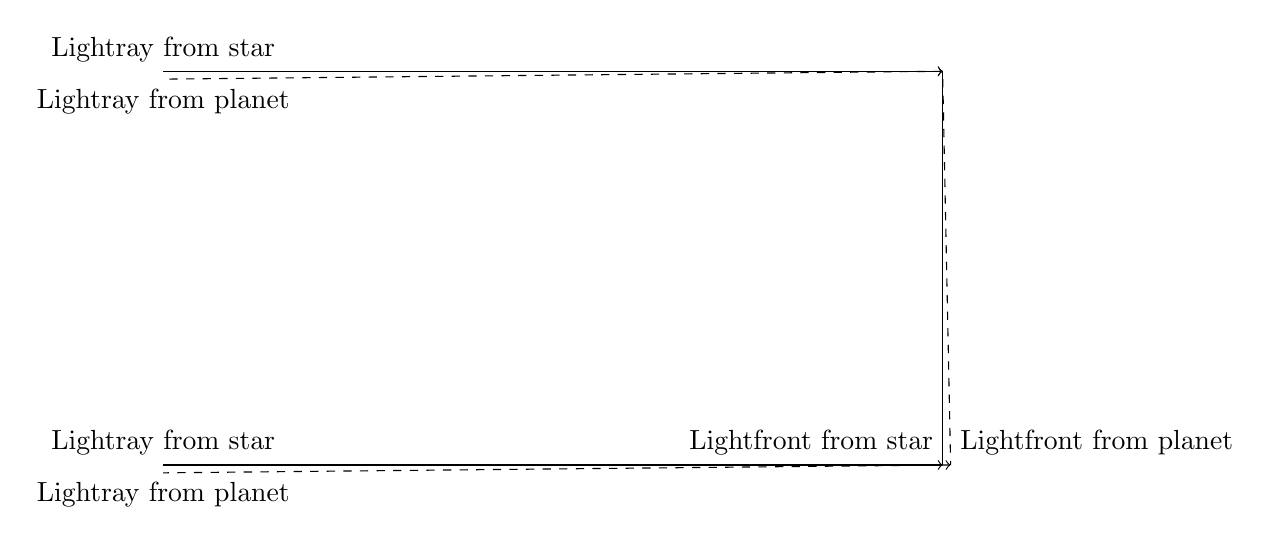
\begin{tikzpicture}(10.5,7)
\draw [line width=0.4pt, <-] (9.9,6)--(0,6) node[above] {Lightray from star};
\draw [dashed, <-] (9.9,6)--(0,5.9) node[below] {Lightray from planet};
\draw [line width=0.4pt, <-] (9.9,1)--(0,1) node[above] {Lightray from star};
\draw [dashed, <-] (10,1)--(0,0.9) node[below] {Lightray from planet};
\draw [line width=0.4pt] (9.9,6)--(9.9,1) node[above left] {Lightfront from star};
\draw [dashed] (9.9,5.9)--(10,1) node[above right] {Lightfront from planet};
\end{tikzpicture}
\caption{Resolution of a telescope.}\label{fig:tel_res}
\end{center}\end{figure}

The smallest angle that can be distinguished with a telescope is:
\begin{equation}
\sin(\alpha) \approx \tan(\alpha) \approx \alpha \approx \frac{\lambda}{\mbox{Diameter}_{\mbox{objective}}}
\end{equation}

The angle between the planet and star can be calculated with (see figure \ref{fig:tel_res}):
\begin{equation}
\alpha = \frac{\mbox{distance}_{\mbox{planet,star}}}{\mbox{distance}_{\mbox{telescope,star}}} 
\end{equation}

\begin{shaded}
\textbf{Exercise \theExercise \stepcounter{Exercise}} : An alien on a planet near $\epsilon$ Eri, distance to our Sun 10.522 light year, builds a telescope and uses it to look at our Sun. The alien sees a small blue planet rotating around the star. What is the distance between Earth and the Sun? What is the wavelength of blue light? Use the answers to the previous questions the calculate the (minimal) diameter of the telescope used by the alien.\end{shaded}
\begin{shaded}
\textbf{Exercise \theExercise \stepcounter{Exercise}} : Estimate the ratio between the light coming from the Sun and the Earth collected by the telescope.\end{shaded}
\begin{shaded}
\textbf{Exercise \theExercise \stepcounter{Exercise}} : Explain if Mars, the red planet, is easier harder to detect by the alien.\end{shaded}
\end{document}


